\documentclass[
	11pt, 
	DIV10,
	ngerman,
	a4paper, 
	oneside, 
	headings=normal, 
	captions=tableheading,
	final, 
	numbers=noenddot
]{scrartcl}

\usepackage{graphicx}
\usepackage{hyperref}


\title{Fully Asynchronous SPH Simulation}
\subtitle{\vspace{0.5cm}Seminar: Current Topics in Fluid Animation}
\author{Yinglun Liu}


\begin{document}
\maketitle


\section{Motivation}

Over the years, the adoption of smoothed particle hydrodynamics(SPH) has developed to become the common pratice when simulating fluids in various scenes. In non-iterative approaches, the physical state of a fluid particle is constantly influenced by its immediate neighborhood and is thus updated in each time step following a few governing equations that enforces the incompressibility of the fluid. In these equations, the computation of new attributes of the current particle requires several times the access to information from its surrounding neighbors. Intuitively, a natural practice would be to, as did many non-iterative SPH solvers, perform global updates to all particles using a single uniform time step. While iterative SPH solvers nowadays generally yield better performances, traditional non-iterative approaches do not seem to lessen in popularity due to the fact that they are easy to implement and suitable for less turbulent fluids.
\par
Be that as it may, a core defect of non-iterative SPH solvers may lie in the lack of efficiency. On one hand, to enforce a constantly negligible density deviation within the fluid, large stiffness parameters are adopted to generate high pressures. Such selection of parameters demands smaller time steps and, in turn, a greater number of iterations for stable and correct particle interations. This can lead to tremendously higher overhead for the generation of visually realistic animation, where tens of millions of particles are included to allow for as fine-grained details as possible. On the other hand, the author made the observation that, while smaller time steps are essential in heavily interacting regions to guarantee stable simulation, in many less complex parts of the fluid a larger time step suffices (see fig. \ref{fig:1}). That is, the maximum possible time step for a particle varies substantially across different regions of the simulation, and it makes less sense to set one global time step for all particles, since it would inevitably be limited by the single particle with the strictest time constraint and lead to much waste of computational power.

\begin{figure}[tb]
	\centering
	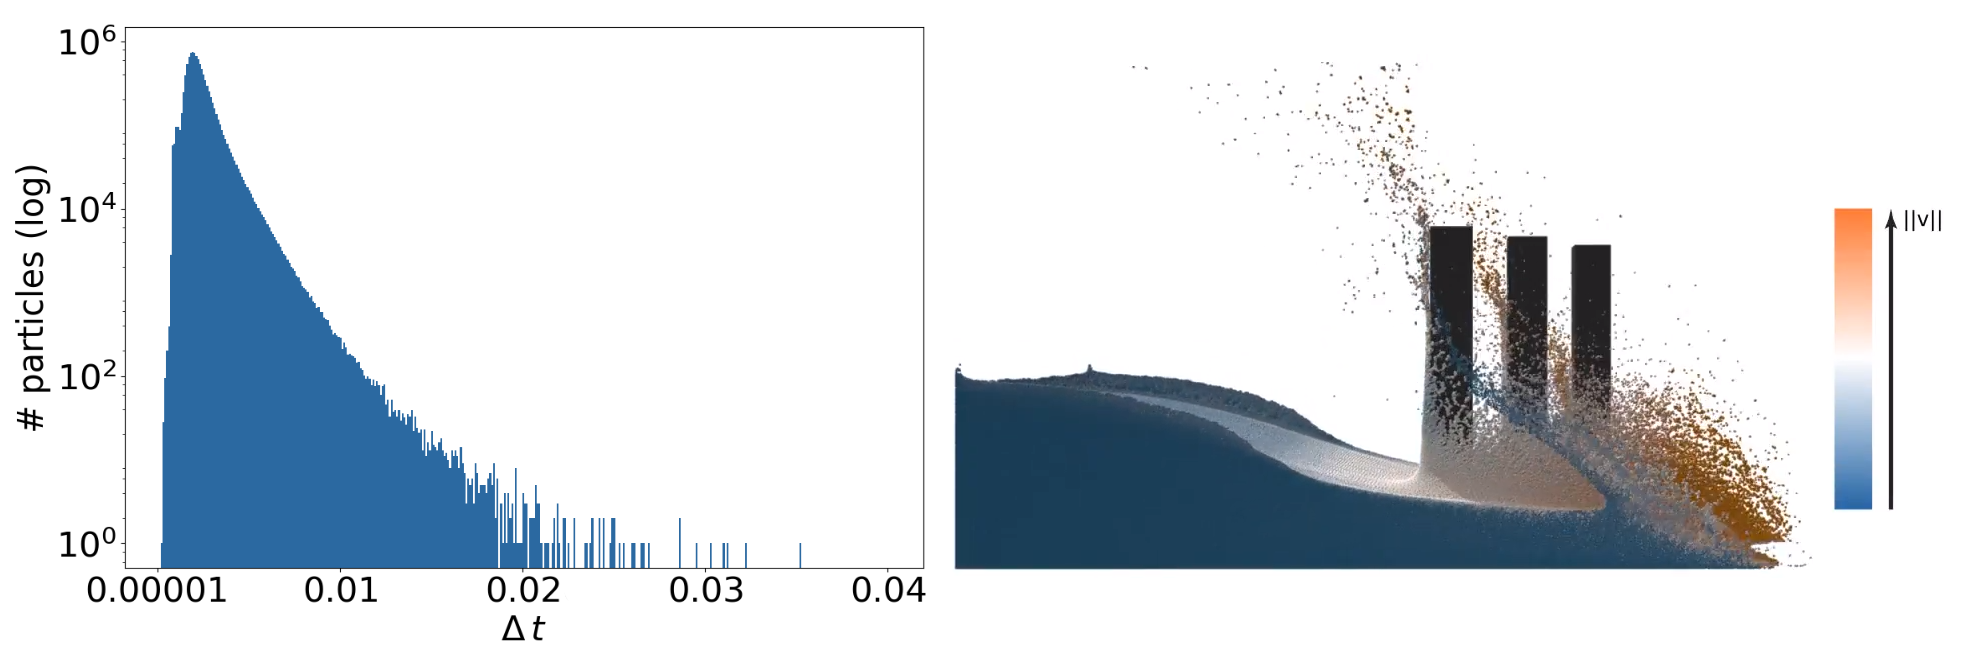
\includegraphics[scale=0.3]{images/1}
	\caption{
		\label{fig:1} For fluid simulation based on SPH, the magnitude of velocity differs substantially 			across particles from different regions (right). As a result, the maximum possible time steps for each 		individual particle could diverge to cover up to multiple magnitudes (left) \cite{reinhardt2017fully}.
	}
\end{figure}

\par
To cope with this, the author proposes a novel method for the time integration of particles, in which each particle is assigned a individual time step and the whole simulation is carried out fully asynchronous. To ensure consistency, the neighborhood is reconstructed at the current time stamp each time a particle is processed. To demonstrate the strength of the proposed method, the author further proposes a multi-queue parallelization to such fully asynchronous integration procedure. Comparative experiments against related works were conducted under diverse conditions and environments to prove the efficacious enhancement on performance.

\section{Related Work}

This is a reference .

\section{Non-iterative SPH}

Governed by the Navier-Stokes equation, non-iterative SPH performs interpolation over the neighborhood of a particle to calculate its attributes and ultimately the forces it incurs within one time step of the simulation. The fluid attribute $ A(x_{i}) $ of particle i at position $ x_{i} $ is computed as the weighted sum of  $ A(x_{j}) $ over all neighboring particles j, with the weights given by a normallizing kernel function W that is of compact support. After all forces are computed, time integration methods like symplectic euler or leap frog is carried out to update particle position and speed.
\par
The author adopts here the splitting strategy as described by \cite{ihmsen2014sph}, where for each update step the advection forces $ F^{advection} $ are separately computed and then used to calculate an intermediate advection velocity $ v^{*} $. An advection density $ \rho^{*} $ is introduced to reflect the expected density at the end of this time step as a result of the divergence in the velocity field if no compensating pressure force is generated. pressures $ p $ pressure forces $ F^{pressure} $ are afterwards handled conventionally. This updating scheme forces the solver to implicitly consider the impact of advection forces before generating pressure forces to counteract the deviation of density and therefore stablizes the simulation. 

\section{Method}

\section{Experiments}

\section{Conclusion}

\bibliographystyle{alpha}
\bibliography{references}

\end{document}          
